\section{PS12, Ex. 1 (A): Job-market signaling}

\begin{frame}{PS12, Ex. 1 (A): Job-market signaling}
  Consider figure 4.2.8 in Gibbons (p. 201). Remind yourselves about the separating equilibrium related to the figure. Why can the high type not choose $e^*(H)$ in a separating equilibrium?\vspace{-8pt}
    \begin{multicols}{2}
      \vfill\null\columnbreak
      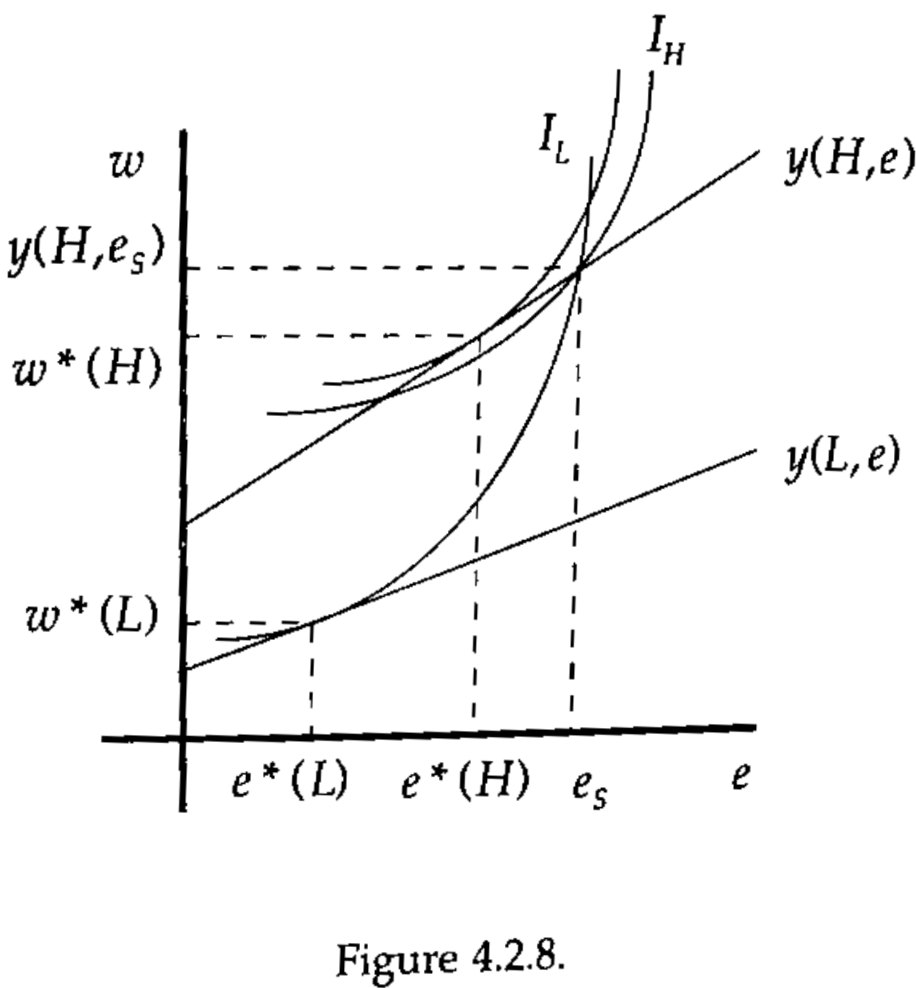
\includegraphics[width=1.1\columnwidth]{figures/Gibbons428}
      \vfill\null
    \end{multicols}
\end{frame}
